%% NOTE: Maximum of 8 pages.

\section{Introduction}\label{intro}

Earthquakes may cause soil rupture or movement, tsunamis and
more. They may cause great losses and that can be explicit by some
examples, such as the earthquakes in Tohoku (2011) and Nepal(2015). To
be able to minimize the consequences of these events, we look to
create forecast earthquake occurences models. Hence the
characteristics that most influence the earthquakes events may vary
both in time and place, these methods should be to adapt their
behavior to be able to forecast earthquakes events which reflects well
the reality.

This project aims to obtain a better method, based in improvements to
the GAModel~\cite{ecta14}, a statistical method of analysis of
earthquakes risk using the Genetic Algorithm technique (GA). Two
ideias are proposed for this. The first one, is to change the
candidate solution representation. By that, we objective to make the
GAModel more specialized, focusing only on areas on which earthquakes
happened already in a near past. This will lead to a faster
convergence, once the amount of parameters is smaller and
consequently, the search space gets smaller.

Formulated on this idea, we propose the ReducedGAModel. Its genome
only has information of areas that already had occurences in the
past. This helps the method to converge gets faster, by minimizing the
number of parameters the method has to deal with.

The other ideia is based on the assumption that earthquakes cluster in
both space and time, and the we want associate the Genetic Algorithm
technique (GA) with a some empirical laws, such as the modified Omori
law. First, the background intensity (the independent earthquakes or
mainshocks), which is a function of the space, is forecasted using the
GA. Then, we use some empirical laws to obtain the dependent
earthquakes (aftershocks) for a specific time interval.

The Emp-GAModel is the method proposed that incorpores some
geophysical knowledge. It is a hybridization of the models generated
by the GAModel with the these empirical laws, see Section
\ref{Models}.

Finally, there is the Emp-ReducedGAModel. This method is a combination
of the two ideias. Therefore, it also performs a hybridization of
models with the group of empirical law. Though, for this method, the
models are generated by the ReducedGAModel method and not by the
GAModel.

The forecast models produced by those methods and the ones produced by
the GAModel were all analyzed using likelihood tests, namely the
L-test, the N-test and the R-test, as suggested by Regional Earthquake
Likelihood Model (RELM)~\cite{schorlemmer2007earthquake}.

For developing the methods and to be able to compare them we used the
earthquake catalog from the Japanese Meteorological Agency (JMA),
using event data from 2005 to 2010.

This paper is organized as: in Section \ref{estadoArte}reviews
applications of Evolutionary Computation in the context of seismology
research. The next Section,Section \ref{Models}, we give a details of
each of the forecast proposed covering the Collaboratory for the Study
of Earthquake Predictability (CSEP) framework and the empirical
laws. In Section \ref{Tests}, we give the description of the tests
proposed in~\cite{Schorlemmer2007}. After that, in \ref{exp}, we
define the target areas used for the experiment and the data from the
JMA; we clarify the design followed during the experiments and how ew
compared the forecast models derived from our methods. Finally, we
show the results and conclude this work in~\ref{Results} and
\ref{Conclusions}.

%TODO: change text to mine version
%TODO: update info + ECTA
\section{Evolutionary Computation for Earthquake Risk Analysis}\label{estadoArte}
In this section we will briefly discuss some reports of the
application of Evolutionary Computation and related method for
Earthquake Risk Analysis.

The usage of Evolutionary Computation in the field of earthquake risk
models is somewhat sporadic. Zhang and Wang~\cite{Zhang2012} used
Genetic Algorithms to fine tune an Artificial Neural Network (ANN) and
use this system to produce a forecast model. Zhou and
Zu~\cite{Feiyan2014} also proposed a combination of ANN and EC, but
their system only forecasts the magnitude parameter of
earthquakes. Sadat, in the paper~\cite{sadat2015application}, follows
the idea oF Zhou and Zu, aiming to predict the magnitude of the
earthquakes in North Iran, but in this case, he used ANN and GA.

Some sismological models were developed aiming to estimate parameter
values by using Evolutionarry Computation. For example, Evolutionary
Computation was used to estimate the peak ground acceleration of
seismically active
areas~\cite{Kermani2009,Cabalar2009,Kerh2010,Kerh2015}. Ramos~\cite{Ramos2011}
used Genetic Algorithms to decide the location of sensing stations and
Saeidian~\cite{saeidian2016evaluation} made a comparation in
performance between the GA and Bees Algorithm to decide which of those
techniques would performe better when chosing the location of sensing
stations. Nicknam et al.~\cite{Nicknam2010} and Kennett and
Sambridge~\cite{Kennett1992} used evolutionary computation to
determine the Fault Model parameters of a earthquake.

%TODO: Last part in somewhat bad
%% CLAUS: A paper to CEC does not need a ``What is EC'' section
%\subsection{What is Evolutionary Computation And What are Genetic Algorithms}\label{EC}
%Evolutionary Computation (EC) is concerned with algorithms based on
%the Darwinian principles of natural selection. It may find, by try
%trial and error and based on a great amount of data, better solutions
%for problems that human beings may not find it easy to
%solve~\cite{koza2003genetic}. That could also be done without any
%domain knowledge about the problem to be
%controlled~\cite{Michie94machinelearning}.
%	
%The main goal of a Genetic Algorithm (GA), a EC technique, is to find
%approximated solutions in problems of search and optimization. Based
%on Koza~\cite{koza2003genetic}, GA are mechanism of search based on
%natural selection and genetic. They explore historical data to find
%optimum search points with some performance
%increment~\cite{Goldberg:1989:GAS:534133}.
%
%A GA uses those mechanisms to generate solutions to optimization and
%search problems. The first step is to create an initial population, a
%group of possible solutions, where each solution is called an
%individual. Those individuals have its fitness value estimated by a
%given function and those with greater fitness value are then chosen to
%reproduction. After some evaluations, we expect to find an optimum
%solution.
%
%Frequently, the initial population is randomly generated once it is
%common to ignore the main aspects that influence the algorithm
%performance. In other words, hence it is common to lack domain
%knowledge, the random population is a good way to start searching for
%optimum solutions.

%TODO: Why 1-year?
\section{The Forecast Models Using Genetic Algorithm}\label{Models}

All forecast models proposed in this paper are based in the
Collaboratory for the Study of Earthquake Predictability (CSEP)
framework.

Each individual has its own representation of the framework based on
different perceptions of what are the best aspects of the framework.

The population is trained on earthquake event data for a training
period, which is anterior to the target test period. After completing
the evaluation limit, the best individual is chosen to be the final
forecast.

\subsection{1-year Models}
The CSEP framework, a forecast model uses a gridded rate
forecast~\cite{zechar2010evaluating}, one common format in the
literature. For this format a geographical region is divided in
sections, bins, during a start date and an end date. The forecast will
estimate the number (and sometimes the magnitude) of earthquakes that
happens in this target region, during the target time interval. For
this study we considered the target time interval of one
year~\cite{ecta14}.

Large and independent earthquakes, also known as mainshocks, are
followed by a wave of others earthquakes, the
aftershocks~\cite{schorlemmer2010first}. Hence there is no physical
measurement to identify mainshocks and its
aftershocks~\cite{schorlemmer2010first}, we divided the forecast
models in two groups: the ones that only forecasts mainshocks and
those that forecast both mainshocks and aftershocks.

Both classes forecast earthquakes with magnitude greater than 3.0 for
every scenario proposed, with a binning of 0.1, here named as cells to
avoid conflicts with the location bin. That results in magnitude cells
of [3.0, 3.1), [3.1, 3.2), until [9.9, 10). That was the only
declustering procudered used for the all methods.

\subsection{Genome Representation}\label{genome}
In the GAModel each individual represents an entire forecast
model. Each gene of the individual is a real value, corresponding to
one bin in the desired model. The values are sampled from the interval
[0, 1). These real values are converted to a integer forecast, we use
  the same modification of the Poisson deviates extraction algorithm
  used for the GAModel~\cite{ecta14}.

In the ReducedGAModel, each individual is a list of a subregion of the
forecast model. This list initially is a refers to bins where
earthquake events happened in the past. During the develop of the
ReducedGAModel, the list may refer to positions that never had
occurrences before. Each element of the list, a gene, also contains
one real value between [0,1). In the initial population, this real
values are sampled from a uniform population. When needed, every
real value is converted to a integer forecast, as in the
GAModel~\cite{ecta14}.

To generate the forecast model we need to do an intermediate step. We
map every location from the list with a bin in the forecast map.

The genome size is usually smaller than the one used in the GAModel
and the Emp-GAModel, once the amount of subregions where earthquakes
with magnitude above 3.0 happened for any given area is smaller then
the total number of genes of the individual.

The Emp-ReducedGAModel and the Emp-GAModel differs only from the
ReducedGAmodel and from the GAmodel, respectively, by the use of
equations after the forecast is provided. This means that the theirs
genome representation are the same as the GAModel and the
ReducedGAModel,correspondingly.

For all methods, the genome is a real valued array X, where each
element corresponds to one bin in the desired model (the number of
bins n is defined by the problem). Each element $x_i \in X$ takes a
value from $[0,1)$. In the initial population, these values are
sampled from a uniform distribution. For more details of the genome
represatation, please refer to~\cite{ecta14}.

\subsection{Fitness Function}
All the methods use the log-likelihood value, for the fitness
function. The fittest individual among all the others, is preserved in
the next generation, to make the solution of one generation as good as
the its last generation.  The bins, a gene of the genome
representation, $b_n$, define the set $\beta$ and $n$ is the size of
the set $\beta$:
\begin{equation} 
\beta := {b_1,b_2,...,b_n},n = |\beta|.
\end{equation}
The probability values of the model $j$, expressed by the symbol
$\Lambda$, is made of expectations $\lambda_i^j$ by bin $b_i$. The
vector is define as:
				
\begin{equation}
	\Lambda^j = 
\begin{pmatrix}
    \lambda_1^j, 
    \lambda_2^j, 
    \hdots,
    \lambda_i^j
  \end{pmatrix}
  ;\lambda_i^j := \lambda_i^j(b_i),b_i \in \beta
\end{equation}
		
The vector of earthquake quantity expectations is defined as:
earthquake by time. The $\Omega$ vector is composed by observations
$\omega_i$ per bin $b_i$, as the $\Lambda$ vector:

\begin{equation}
\Omega = 
\begin{pmatrix}
    \omega_1,
    \omega_2,
    \hdots,
    \omega_i
  \end{pmatrix}
  ;\omega_i =\omega_i(b_i),b_i \in \beta
\end{equation}

The calculation of the log-likelihood value for the $\omega_i$
observation with a given expectation $\lambda$ is defined as:


\begin{equation}
	L(\omega_i|\lambda_i^j) = -\lambda_i^j + \omega_i\log\lambda_i^j - \log\omega_i!
\end{equation}

The joint probability is the product of the likelihood of each bin, so
the logarithm $L(\Omega|\Lambda^j)$ is the sum of for
$L(\omega_i|\lambda_i^j)$ every bin $b_i$:

\begin{equation}\label{log-like}
\begin{split}
	L^j = L(\Omega|\Lambda^j) = \sum_{i=1}^{n}L(\omega_i|\lambda_i^j)  \\
	= \sum_{i=1}^{n} -\lambda_i^j + \omega_i\log\lambda_i^j - \log\omega_i!  
\end{split}
\end{equation}

The fitness function is a coded version of the equation
~\ref{log-like}. It uses the probabilities of the bins of each
individual of model for the $\lambda$ values.

\subsection{Evolutionary Operators}
Both the GAModel and the Emp-GAModel use a combination of operators
made available by the Distributed Evolutionary Algorithms in Python
(DEAP)~\cite{DeRainville:2012:DPF:2330784.2330799}. We used the One
Point Crossover for the crossover operator, the Polynomial Bounded
Mutation for the mutation operator and for selection, we used
Tournament selection and Elitism. The parameters are described in the
Table~\ref{GAParameters}.

\begin{table}[!ht]
  \caption{Parameters used in GAModel and Emp-GAModel}
  \label{GAParameters}
  \begin{center}
  \begin{tabular}{|l|r|}
    \hline
    Population Size & 500\\
    Generation Number & 100\\
    Elite Size & 1\\
    Tournament Size & 3\\
    Crossover Chance & 0.9\\
    Mutation Chance (individual) & 0.1\\
	Polynomial Bounded parameters & eta = 1, low = 0, up = 1\\
    \hline    
  \end{tabular}
  \end{center}
\end{table}

For the ReducedGAModel and the Emp-ReducedGAModel, the only different
operator is the mutation fuction. We use a simple mutation operator
which samples entirely two new values, both sampled from uniform
distributions. The first, is a new real value from [0,1) and the
seconde one, a new integer value from [0,X), where X is the maximum
length of the genome. For the parameters see
Table~\ref{GAHParameters}.

\begin{table}[!ht]
  \caption{Parameters used in GAModel and Emp-GAModel}
  \label{GAHParameters}
  \begin{center}
  \begin{tabular}{|l|r|}
    \hline
    Population Size & 500\\
    Generation Number & 100\\
    Elite Size & 1\\
    Tournament Size & 3\\
    Crossover Chance & 0.9\\
    Mutation Chance (individual) & 0.1\\
    \hline    
  \end{tabular}
  \end{center}
\end{table}

\subsection{Mainshock Models}
The GAModel is completely based on the framework suggested by the
CSEP. In it, one forecast is defined as a region in a specfic time
interval and is divided in bins. Each bin represents a geographical
interval. The whole target area of study is covered by a group of
these bins where each bin has an earthquake forecast value. This
groups of bin represent the $\mu(x,y)$, the background
intensity~\cite{zhuang2004analyzing}. In the GAModel, each possible
solution is represented as an entire forecast model.

In this context the GAModel is considered as one method to generate
space-rate-time forecasts. It also could be described as:
\begin{equation}\label{gamodel}
 \Lambda(t,x,y,M|\Upsilon_t) = \mu(x,y)
\end{equation}
where you can denote the number of earthquakes forecast in all bins 
as $\Lambda(t,x,y)$~\cite{zechar2010evaluating} given that $\Upsilon_t$ 
is the earthquake observation data up to time $t$.


% Which leads to $\mu(x,y)$ the background intensity, a function of
% space, but not of time~\cite{zhuang2004analyzing}.

The ReducedGAModel, which represents the idea of changing the
candidates solution representation (see Section~\ref{intro}), is a
method with a similar description of the GAModel. The difference is
that, in the ReducedGAModel each possible solution represents only a
fraction of the forecast where we expect to find especific risk areas.

The GAModel defines a expected number of earthquakes for every single
bin in the target region. That could lead to exhaustive and, sometimes
worthless, searches. That is caused by the number of bins in the
forecast and also because some in some bins there are no earthquake
occurances in the observation data. To minimize this, the
ReducedGAModel only define expected number of earthquakes in bins that
already had some occurance in the past, giving a direction to where
the GA should search.

To make it clear, we use the same example as the one used
in~\cite{ecta14}. The "Kanto" region, one of the four areas used in
both studies, is divided into 2025 bins (a grid of 45x45
squares). Each bin has an area of approximately $25km^2$. The GAModel
then calculates an expected number of earthquakes for every bin on a
determinated time interval, so the GA searches for good values in 2025
bins.

The ReducedGAModel will first obtain the position of past
occurances. Then it will calculate some expected number of earthquakes
only for the bins related to those positions. During the development
of this method, these positions may vary, including positions that
never had earthquake events before. That is important to add some
variation to the method. For example, if there are 10 bins with
occurances in "Kanto" in the last year, it will make the GA start
searching for good values for only those 10 bins, leaving the other
2015 bins empty, representing zero occurances. It is important to
highlight that in the worst case, it will make the same amount of
searches as the GAModel. The final forecast model will maintain the
amount of bins with occurrance, but the number of events for every bin
and their location may change.

% (it is possible that an bin had more the one occurance, therefore that number will drop. 

\subsection{Mainshock+Aftershock Models}
Hence earthquakes cluster in space and inspired by the space-time
epidemic-type aftershock sequence (ETAS), the Emp-GAModel, represents
the ideia of associating the GA with empirical laws (see
Section~\ref{intro}). It is described as:

\begin{equation}\label{reducedgamodel}
	\Lambda(t,x,y,M|\Upsilon_t) = \mu(x,y)J(M)
\end{equation}


\begin{equation}\label{emp-model}
 \Lambda(t,x,y|\Upsilon_t) = \mu(x,y) + \displaystyle\sum_{t_i \in t} K(M_i)g(t-t_i)P(x,y)
\end{equation}
%TODO: explicar o Upsilon

The Emp-GAModel uses $\mu(x,y)$ as defined for the GAModel, so it
calculates an expected number of earthquakes for every bin in the
target region. P(x,y) calculates the position of the aftershocks with base on the origin of the mainshock. It is a simple space distribuition function, that alocates the aftershocks in one of the following posotions: upper, lower, left or right. It runs for a number of steps, getting futter from the origin at each step or as when there are no more events to be alocated. The Omori law, $g(t)$, which is considered one
empirical formula of great
success~\cite{zhuang2004analyzing}~\cite{utsu1995centenary}~\cite{omori1895after},
is a power law that relates the earthquake occurance and its magnitude
with the decay of aftershocks activity with time. For this approach we
used the probabilty density function (pdf) form of the modifed Omori
law~\cite{zhuang2004analyzing}:

\begin{equation}\label{omori}
	g(t)= \dfrac{(p-1)}{c(1+ \dfrac{t}{c})^(-p)}
\end{equation}

In the paper~\cite{utsu1995centenary}, Utsu says that most p and c
values, for various earthquake data sets fall in the range between 0.9
and 1.4, and between 0.003 and 0.3 days, respectively. These values
were based on the Davidon-Fletcher-Powell optimization procedure and
used in ETAS~\cite{utsu1995centenary}.

Based on paper~\cite{yamanaka1990scaling}, we set the values of $1.3$
for $p$ and $0.003$ for $c$ for our the experiments. Following the
statement make in this report, we set the time interval $t$ between a
mainshock and its aftershocks at one month. The statement says that if
the $t$ value is too short, the number of aftershocks is too small,
but if it is too big, we may also consider background activity.

For $K(M_i)$, the total amount of triggered events, we count
aftershocks within a given area, $A$, using the following formula,
where $M_c$ is the magnitude threshold:

\begin{equation}\label{triggered}
 K(M_i) = A\ exp([\alpha(M-M_c)])
\end{equation}

In the paper~\cite{ogata2006space}, it states that $\alpha$ should be
equal to the inverse of the magnitude of an event, or
$magnitide^{-1}$. To obtain $A$, the following equation
from~\cite{yamanaka1990scaling}, was used:

\begin{equation}
A = e^{(1.02M -4)}
\end{equation}



%TODO: maybe no
and lastly, the $J(M)$ is a simulation of the event magnitude by
Gutenberg-Richter's Law, using Add SAPP
% $1$ as the value of $\beta$ ~\cite{helmstetter2003predictability}:
%
%\begin{equation}\label{gut-ritcher}
%J(M) = \beta e^{-\beta(M-M_c)}, M \geq M_c
%\end{equation}

At last, the Emp-ReducedGAModel is a mix between the ideas in the
ReducedGAModel method and the Emp-GAModel, which means that its genome
representation is equal to the Emp-GAModel but its candidates have
same list of locations format, as in the ReducedGAModel.

%TODO: Move this whole section to exp (where there?)
\section{Tests for evaluating Models}\label{Tests}

In the paper {\it Earthquake Likelihood Model
  Testing}~\cite{schorlemmer2007earthquake}, it is proposed some
statistical tests that are used in this study, developed by the The
Regional Earthquake Likelihood Models (RELM).They were used to compare
and evaluate the every forecast models. These tests are based on the
log-likelihood score that compares the probability of the model with
the observed events.

To evalute the data-consistency of the forecast models we used the
N-Test, the Number Test, and the L-Test, or Likelihood Test. These
tests fall are significance tests. Therfore, assuming a given forecast
model as the null hypothesys, the distribuition of an observable test
is simulated. If the observed test statistic falls into the upper or
lower tail of this distribuition, the forecast is
rejected~\cite{schorlemmer2010first}.

To be able to compare the model that passed the N-Test and the L-test,
the R-Test, the hypotheses Comparison Test, is used. It calculates the
relative performance of a model, by comparing the Log-likelihood
values between two forecast models.

\subsection{Likelihood Test or L-Test}
 
The L(ikelihood) Test considers that the likelihood value of the model
is consistent with the value obtain with the simulations. The value is
calculated by the formula, where $\widehat{L}_k$ is the value of the
Log-likelihood of the model {\it j}, in the {\it bin} {\it i} and
$\widetilde{L}$ is the value of the Log-likelihood of the simulation
{\it j} in the {\it bin} {\it q}:


\begin{equation}
\gamma^{j}_{q} = \frac{\left| \left\{ \widehat{L}^j_k | \widehat{L}^j_k \leq \widetilde{L}^j_q, \widehat{L}^j_k \in \widehat{L}^j, \widetilde{L}^j_q \in \widetilde{L}^j  \right\} \right|}  {|\widehat{L}^j|}
\end{equation}

The analisys of the results can be splited into 3 categories, as follows:

\begin{enumerate}
\item Case 1: $\gamma^{j}$ is a low value, or in other words, the
  Log-likelihood of the model is lower then most of the Log-likelihood
  of the simulations. In this case, the model is rejected.
\item Case 2: $\gamma^{j}$ falls near the half of the values obtained
  from the simluations and is consistent with the data.
\item Case 3: $\gamma^{j}$ is high. This means that the Log-likelihood
  of the data da is higher that the Log-likelihood of the model and no
  conclusion can be made what so ever.
\end{enumerate}


It is important to highlight that no model should be reject in case 3,
if based only on the L-Test. In this case the consistency can or
cannot be real, therefore these model should be tested by the N-Test
so that further conclusions can be done.

\subsection{Number test or N-Test}
The N(umber)-Test also analises the consistency of the model, but it
compares the number os observations with the number of events of the
simulations. This test is necessary to supply the underpredicting
problem, which may pass unnoticed by the L-Test.

This mesure is estimated by the fraction of the total number of
observations by the total number of observations of the model.

As the L-test, if the number of events falls near the half of the
values of the distruition, then the model is consistent with the
observation, nor estimating too much events nor too few of them.

\subsection{Hypotheses Comparison Test or R-Test}

The Hypotheses Comparison, or the R(atio)-Test, compares two forecast
models against themselves. The log-likelihood is calculted for both
models and then the difference between them is calculated, named the
observed likelihood ratio. This value indicates which one of the model
better fits the observations.

The likelihood ratio is calculated for each simulated catalog. If the
fraction of simulated likelihood ratios less than the observed
likelihood ratio is very small, the model is reject.  To make this
test impartial, not given an advantage to any model, this procedure is
applied symmetrically~\cite{schorlemmer2010first}.


\subsection{Evaluation}\label{eval}
The evaluation process is made as follow: First, the data-consitency
is tested by the L-Test and the R-test. If the model passes these
tests, meaning that it was not rejected by them, they ares compared
with other forecast models, which were also not reject, with the
R-Test. The model that best fits the R-Test is then chose as the best
model~\cite{schorlemmer2007earthquake}.

%data, design, comparacao, regions, year(s)
%para o só ga ,boxplot e t-test tem que ver se tem vantagem
%para com equations usar os testes
\section{Experiments}\label{exp}
%Tuned configuration: A parameter configuration tuned for the smaller
%budget of 500 evaluations used in this experiment. The tuned
%parameter values for each algorithm were calculated using the
%Sequential Model-based Algorithm Configuration method (SMAC) [7].

To analyze the performance of the forecasts generated by the GAModel,
the ReducedGAModel, the Emp-GAModel and finally the
Emp-ReducedGAModel, we perfom a simulation. All methods use the folling 
simulation structure. First, all method evolve using a training data set,
then the resulting forecast is analysed against a test data set.

To analise the resulting forecast two evaluation methods were performed.
 One of the method is the evaluation method proposed by~\cite{schorlemmer2007earthquake}
 and described in Section~\ref{eval}. The other method is the Student's t-test, a statistical hypothesys test, that we use to determine if two models are significantly different from each other.

The data of the JMA catalog was divided into four
groups objecting a better understand of the patterns that most influence the
earthquakes events and also to be able to determine the qualities of
those forecasts. Each group contains only of earthquakes that happened in a
specific time interval for a given area of Japan. The experimental
data will be described in details subsequently.

\subsection{Experimental Data}
The data used in these experiments comes from the Japan Meteorological
Agency's (JMA) catalog. It is a list of earthquakes events which took
place in Japan from 2000 to 2013. Each event is characterized by some
typical earhtquake information such as magnitude, latitude, longitude,
and depth.

For the experiments we consider events with magnitude above 3.0 which
happened in four specific areas of Japan, during the year of
???. Those areas (Kanto, Tohoku, Kansai and East Japan) represent
different earthquake attributes and could lead to more information
about the power of the forecasts and/or its pitfalls. Kanto, Touhoku
and Kansai contain mainly inland earthquakes, which are considered to
follow more stable pattern. Figure~\ref{areamap} shows the locations of these four areas. East Japan includes also many off-shore earthquakes. For more information about the four regions please refer to~\cite{ecta14}.

\begin{figure}
  \begin{center}
  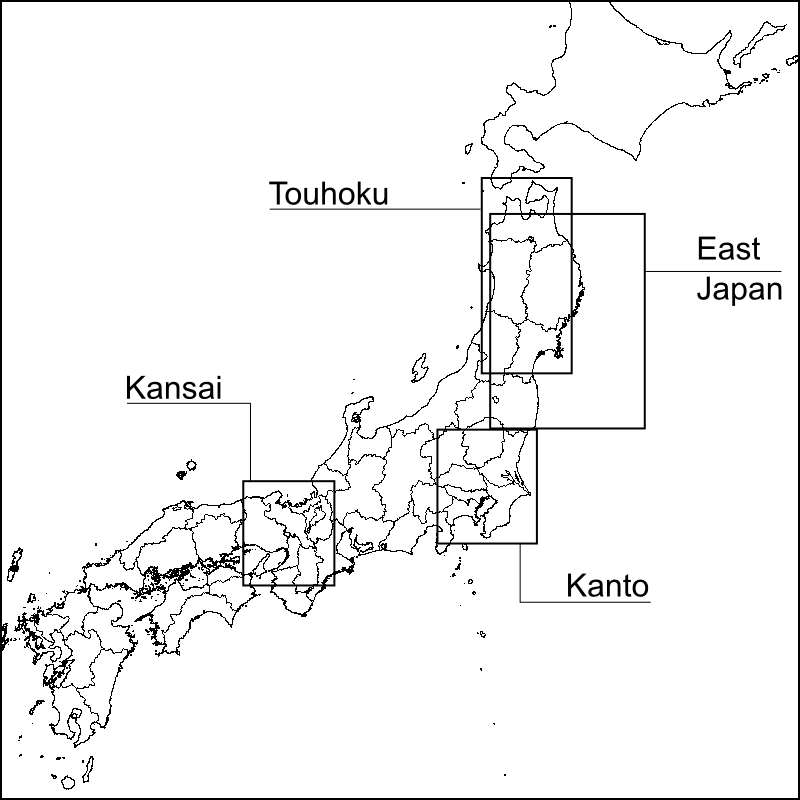
\includegraphics[width=0.40\textwidth]{img/alljapan.png}
  \end{center}
  \caption{The relative locations of the four areas used in our
    experiments}
  \label{areamap}
\end{figure}

% Kanto: Kanto is the area at and nearby Tokyo. There is a large
%amount of seismic activity in the target period. In this study, we
%define this region as starting at N34.8,W138.8, with 2025 bins ar-
%ranged in a 45x45 grid. Each bin corresponds to a 5km2 square.

%Kansai: The Kansai area includes Kyoto, Osaka, Kobe and nearby
%cities. This area shows a rela- tively lower amount of seismic
%activity in the pe- riod considered. We define this region as start-
%ing at N34,W134.5, with 1600 bins arranged in a 40x40 grid. Each bin
%corresponds to a 5km2 square.

%Touhoku: The Touhoku region is defined as the northern provinces of
%the main island. It shows some clusters of seismic activity during
%the pe- riod studied. We define this region as starting at
%N37.8,W139.8, with 800 bins arranged in a 40x20 grid. Each bin
%corresponds to a 10km2 square.

%East Japan: This area corresponds to Japan’s north-eastern coast. It
%includes both inland and off-shore events, which makes it more
%difficult to forecast. It also includes the location of the M9
%earthquake of 2011. We define this region as starting at N37,W140,
%with 1600 bins arranged in a 40x40 grid. Each bin corresponds to a
%10km2 square.

\subsection{Experimental Design}
To compare the performance of the forecast models, we execute a
simulation experiment on ??? scenarios. Each scenario is defined by a
region for a 1-year interval, starting in Jan/01 and ending in
Dec/31. To build one scenario, one region is chosen from the set of
regions (Kanto, Tohoku, East Japan and Kansai) for a determinated
year. To train the methods, we use 5 years of prior data set. For example,
to train the 1-year GAModel forecast model for the year of 2010 in Kanto region, the data used is from the events which occurred in the years of 2006, 2007, 2008 and 2009 in
Kanto. This pattern is the same for all methods.

To compare the results of the forecasts models, we used two approaches. The first
one is based on the evaluation method proposed
by~\cite{Schorlemmer2007} and used in~\cite{schorlemmer2010first}. As
described in~\ref{eval}, the forecasts were first analysed using the
L- and N- test and ??????  was chosen by the R-test as the recommended
one.

The second approach is to use the Log-likelihood values obtained by
each of the forecast for each scenario. The log likelihood indicates
how close the forecast is to the test data, in terms of location and
quantity of earthquakes~\cite{ecta14}.

All methods presented here are stochastic methods. Therefore,
to be able to compare and test the statistical significance of the
results, we run each forecast model 20 times. This signifies that all
results showed are the mean of these 20 executions.

%\subsection{Parameter Tuning}
%%All 4 algorithms were tuned using the Sequential Model- based
%%Algorithm Configuration, SMAC [7].
%

%Parameter tunning is a commonly practiced approach which aims to find
%optimum parameters values before the run of a algorithm. Later this
%algorithm is executed with these values, which remain fixed during
%the run~\cite{eiben2011parameter}.

%%review this
%To find a good set of parameters for the all the forecast models
%algorithms, the pySMAC, a Python wrapper for the hyperparameter
%optimization tool Sequential Model- based Algorithm Configuration
%(SMAC)~\cite{hutter2010sequential}, was used.

%SMAC is an algorithm configurator takes as input an algorithm
%executable, a formal description of the parameters for the algorithm,
%and a set of training problem instances. It searches the space of
%possible parameter values by generating a candidate configuration and
%evaluating the configuration on the set of the training
%instances~\cite{aranha2015optimization}.

%The configuration which best fits each one of the forecast models
%algorithm is then chosen to be used as the set of values for the its
%algorithms run. For all algorithms present here, the default control
%parameter values (which are based on the values applied in the
%GAModel~\cite{ecta14}), the ranges for the parameters (arbitrarily
%chosen), as well as the values found by SMAC, are shown in
%Table~\ref{smac-par} for GAModel and Emp-GAmodel and in
%Table~\ref{smac-par2} for ReducedGAModel and Emp-ReducedGAModel.

%EXPLICAR A QUESTAO DA EXPLICACAO DOS PARAMETROS $N_GEN * POP = CONST$
%
%
%\begin{table}[!h]
%  \begin{center}
%  \caption{The default control parameter values and the best set of parameters found by tunning the algorithm with SMAC for the ReducedGAModel and the Emp-ReducedGAModel}
%\begin{tabular}{ |c|c|c|c|c| }
%\hline
%%\multicolumn{5}{ |c| }{SMAC configuration and values for GAModel and Emp-GAModel} \\
%\hline
%\multirow{5}{*}{Kanto}
% & Parameter & Range & Default & Tuned \\
% \cline{2-5}
% & Crossover Chance & [0,1] & 0.9 & 0.9\\
% & Mutation Chance & [0,1] & 0.1 & 0.1\\
% & Population Size & N/A & 500 &\\
% & Generation Number & [50,250] & 100 & 100 \\ \hline
%\multirow{4}{*}{Kansai}
% & Parameter & Range & Default & Tuned \\
% \cline{2-5}
% & Crossover Chance & [0,1] & 0.9 & 0.9\\
% & Mutation Chance & [0,1] & 0.1 & 0.1\\
% & Population Size & N/A & 500 &\\\ 
% & Generation Number & [50,250] & 100 & 100 \\ \hline
%\multirow{4}{*}{Tohoku}
% & Parameter & Range & Default & Tuned \\
% \cline{2-5}
% & Crossover Chance & [0,1] & 0.9 & 0.9\\
% & Mutation Chance & [0,1] & 0.1 & 0.1\\
% & Population Size & N/A & 500 &\\
% & Generation Number & [50,250] & 100 & 100 \\ \hline
%\multirow{4}{*}{East Japan}
% & Parameter & Range & Default & Tuned \\
% \cline{2-5}
% & Crossover Chance & [0,1] & 0.9 & 0.8826\\
% & Mutation Chance & [0,1] & 0.1 & 0.1724\\
% & Population Size & N/A & 500 &\\
% & Generation Number & [50,250] & 100 & 106 \\ \hline
%\hline
%\end{tabular}
%  \end{center}
%  \label{smac-par2}
%\end{table}
%
%\begin{table}[!h]
%  \begin{center}
%  \caption{The default control parameter values and the best set of parameters found by tunning the algorithm with SMAC for the ReducedGAModel and the Emp-ReducedGAModel}
%\begin{tabular}{ |c|c|c|c|c| }
%\hline
%%\multicolumn{5}{ |c| }{SMAC configuration and values for GAModel and Emp-GAModel} \\
%\hline
%\multirow{5}{*}{Kanto}
% & Parameter & Range & Default & Tuned \\
% \cline{2-5}
% & Crossover Chance & [0,1] & 0.9 & 0.9\\
% & Mutation Chance & [0,1] & 0.1 & 0.1\\
% & Population Size & N/A & 500 &\\
% & Generation Number & [50,250] & 100 & 100 \\ \hline
%\multirow{4}{*}{Kansai}
% & Parameter & Range & Default & Tuned \\
% \cline{2-5}
% & Crossover Chance & [0,1] & 0.9 & 0.9\\
% & Mutation Chance & [0,1] & 0.1 & 0.1\\
% & Population Size & N/A & 500 &\\\ 
% & Generation Number & [50,250] & 100 & 100 \\ \hline
%\multirow{4}{*}{Tohoku}
% & Parameter & Range & Default & Tuned \\
% \cline{2-5}
% & Crossover Chance & [0,1] & 0.9 & 0.9\\
% & Mutation Chance & [0,1] & 0.1 & 0.1\\
% & Population Size & N/A & 500 &\\
% & Generation Number & [50,250] & 100 & 100 \\ \hline
%\multirow{4}{*}{East Japan}
% & Parameter & Range & Default & Tuned \\
% \cline{2-5}
% & Crossover Chance & [0,1] & 0.9 & 0.8826\\
% & Mutation Chance & [0,1] & 0.1 & 0.1724\\
% & Population Size & N/A & 500 &\\
% & Generation Number & [50,250] & 100 & 106 \\ \hline
%\hline
%\end{tabular}
%  \end{center}
%  \label{smac-par2}
%\end{table}


%5 https://github.com/automl/pysmac

%TODO: tabelas, imagens, add
%TODO: Discussion of the results, what should i do? is it good?...?
\section{Results}\label{Results}

\begin{figure}[!htb]
\centering
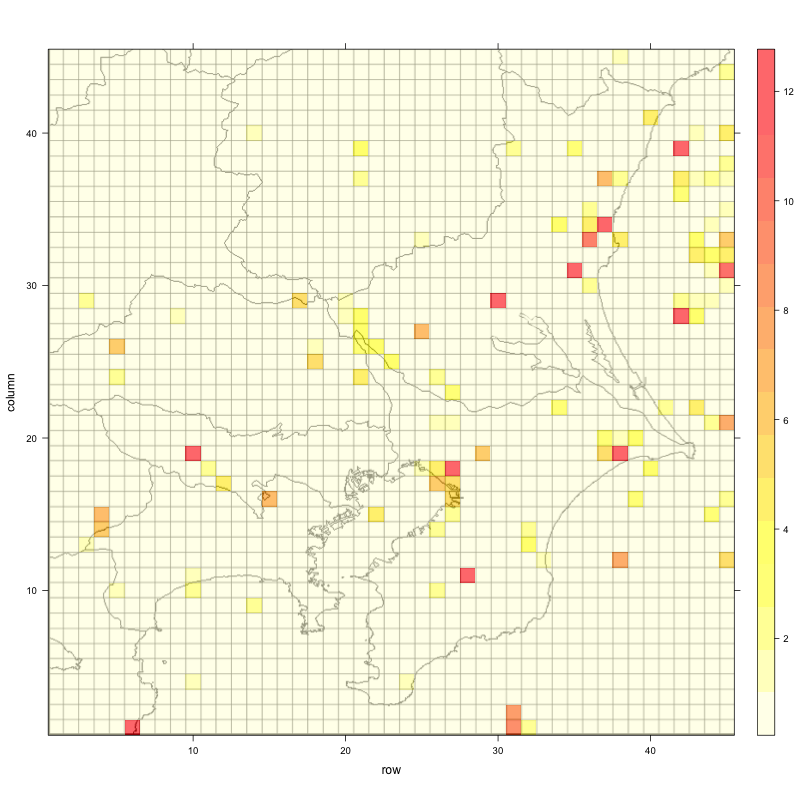
\includegraphics[scale=0.2]{img/NPKanto_2009.png}
\caption{Reduced-Gamodel model for the year of 2009 in Kanto.}
\label{listas-NPKanto_2009.png}
\end{figure}

\begin{figure}[!htb]
\centering
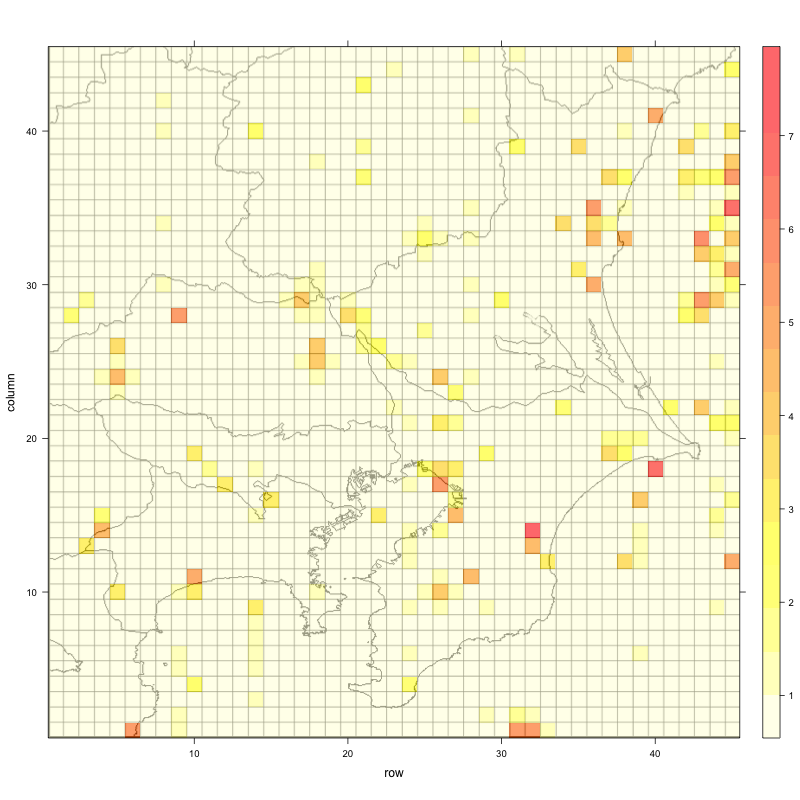
\includegraphics[scale=0.2]{img/modelo_HybridKanto_2009.png}
\caption{Emp-GAModel model for the year of 2009 in Kanto.}
\label{gamodelHybridKanto_2009.png}
\end{figure}

\begin{figure}[!htb]
\centering
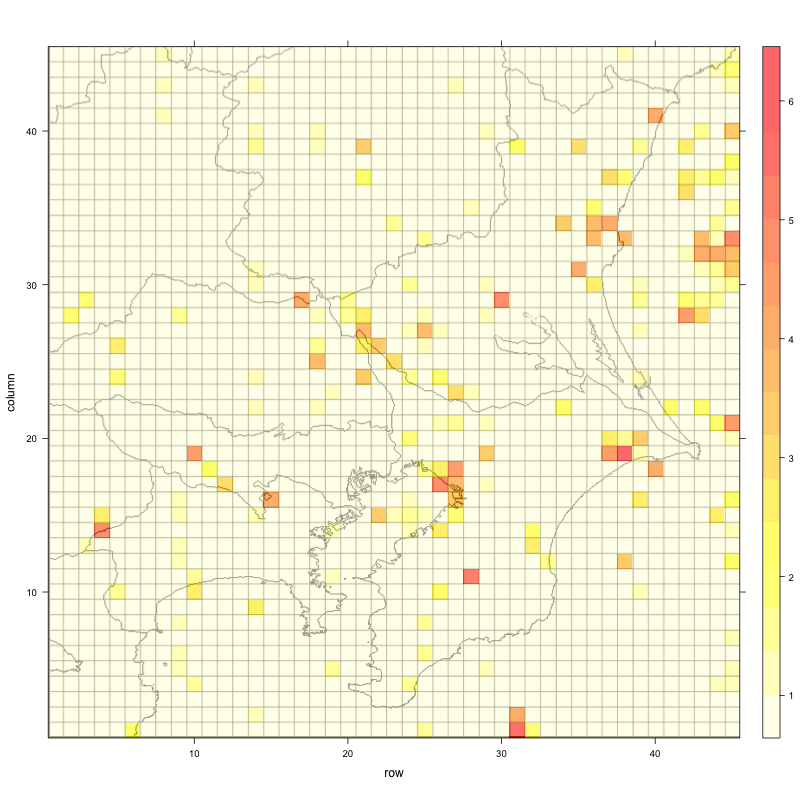
\includegraphics[scale=0.2]{img/NP_HybridKanto_2009.png}
\caption{Emp-ReducedGAModel model for the year of 2009 in Kanto.}
\label{listas-NPHybridKanto_2009.png}
\end{figure}


\begin{figure}[!htb]
\centering
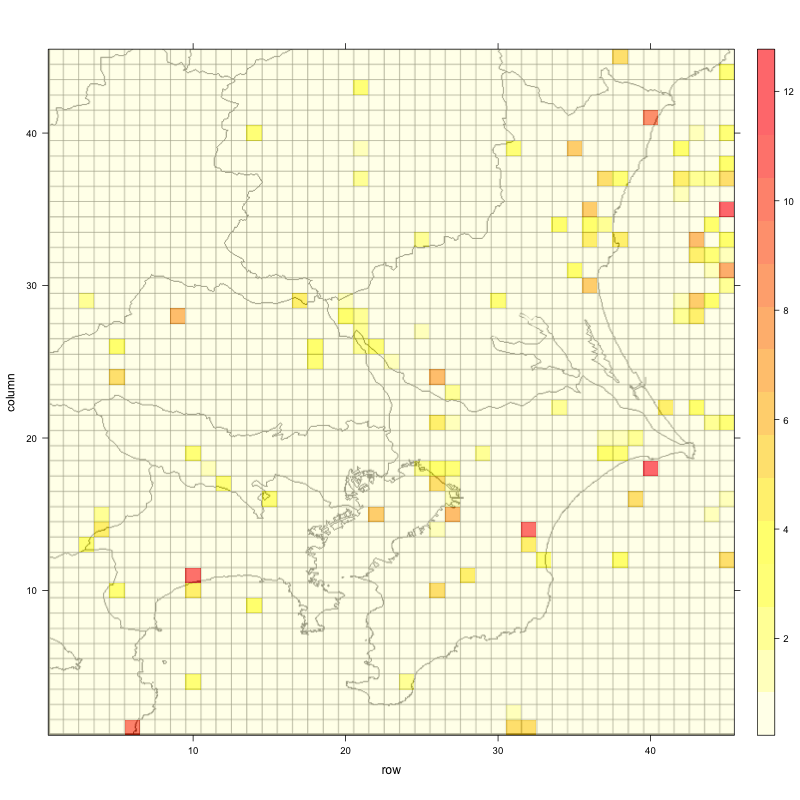
\includegraphics[scale=0.2]{img/modeloKanto_2009.png}
\caption{GAModel model for the year of 2009 in Kanto.}
\label{gamodel_2009.png}
\end{figure}


%TODO: add future work with Gabriels
%TODO: this section should be a revision of all
\section{Conclusions}\label{Conclusions}
%\end{document}  % This is where a 'short' article might terminate

%ACKNOWLEDGMENTS are optional
\section*{Acknowledgments}
The authors would like to thank Bogdan M. Enescu, from the department
of Earth Evolution Sciences in the university of Tsukuba for his
useful comments. 

We would also like to thank the Japan Meteorological Agency for the
earthquake catalog used in this study.
